\documentclass[crop,tikz]{standalone}

\usepackage{pgfplots}
\tikzset{>=latex}
\colorlet{green}{black!40!green}

\pgfplotsset{
  inverted/.style = {
    every axis legend/.append style={
      draw=white,
      fill=hardblack,
      text=white
    }
  }
}

\begin{document}
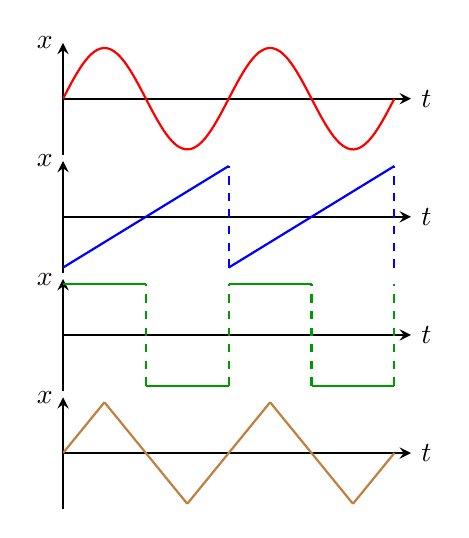
\begin{tikzpicture}
\begin{axis}[
  thick,
  width=6cm,
  height=3cm,
  domain={0}:{4*pi},
  samples=50,
  axis y line=middle,
  axis x line=middle,
  xlabel={$t$},
  ylabel={$x$},
  xlabel style={right},
  ylabel style={left},
  xmin=0, xmax={4.2*pi},
  ymin=-1.1, ymax=1.1,
  xtick={\empty},
  xticklabels={\empty},
  ytick={\empty},
  yticklabels={\empty},
  ]
  \addplot[red,smooth] { sin(deg(x)) };
\end{axis}
%
\begin{axis}[
  thick,
  width=6cm,
  height=3cm,
  samples=50,
  axis y line=middle,
  axis x line=middle,
  xlabel={$t$},
  ylabel={$x$},
  xlabel style={right},
  ylabel style={left},
  xmin=0, xmax={4.2*pi},
  ymin=-1.1, ymax=1.1,
  xtick={\empty},
  xticklabels={\empty},
  ytick={\empty},
  yticklabels={\empty},
  at={(0,-1.5cm)},
  ]
  \addplot[blue,smooth,domain=0:{2*pi}] { x/(pi)-1 };
  \draw[blue,dashed] (axis cs:2*pi,-1) -- (axis cs:2*pi,1);
  \addplot[blue,smooth,domain={2*pi}:{4*pi}] { (x-2*pi)/(pi)-1 };
  \draw[blue,dashed] (axis cs:4*pi,-1) -- (axis cs:4*pi,1);
\end{axis}
%
\begin{axis}[
  thick,
  width=6cm,
  height=3cm,
  samples=50,
  axis y line=middle,
  axis x line=middle,
  xlabel={$t$},
  ylabel={$x$},
  xlabel style={right},
  ylabel style={left},
  xmin=0, xmax={4.2*pi},
  ymin=-1.1, ymax=1.1,
  xtick={\empty},
  xticklabels={\empty},
  ytick={\empty},
  yticklabels={\empty},
  at={(0,-3cm)},
  ]
  \addplot[green,smooth,domain=0:{pi}] { 1 };
  \draw[green,dashed] (axis cs:pi,-1) -- (axis cs:pi,1);
  \addplot[green,smooth,domain={pi}:{2*pi}] { -1 };
  \draw[green,dashed] (axis cs:2*pi,-1) -- (axis cs:2*pi,1);
  \addplot[green,smooth,domain={2*pi}:{3*pi}] { 1 };
  \draw[green,dashed] (axis cs:3*pi,-1) -- (axis cs:3*pi,1);
  \addplot[green,smooth,domain={3*pi}:{4*pi}] { -1 };
  \draw[green,dashed] (axis cs:4*pi,-1) -- (axis cs:4*pi,1);
\end{axis}
%
\begin{axis}[
  thick,
  width=6cm,
  height=3cm,
  samples=50,
  axis y line=middle,
  axis x line=middle,
  xlabel={$t$},
  ylabel={$x$},
  xlabel style={right},
  ylabel style={left},
  xmin=0, xmax={4.2*pi},
  ymin=-1.1, ymax=1.1,
  xtick={\empty},
  xticklabels={\empty},
  ytick={\empty},
  yticklabels={\empty},
  at={(0,-4.5cm)},
  ]
  \addplot[brown,smooth,domain=0:{pi/2}         ] { +x/(pi/2)+0 };
  \addplot[brown,smooth,domain={pi/2}:{3/2*pi}  ] { -x/(pi/2)+2 };
  \addplot[brown,smooth,domain={3/2*pi}:{5/2*pi}] { +x/(pi/2)-4 };
  \addplot[brown,smooth,domain={5/2*pi}:{7/2*pi}] { -x/(pi/2)+6 };
  \addplot[brown,smooth,domain={7/2*pi}:{4*pi}  ] { +x/(pi/2)-8 };
\end{axis}
\end{tikzpicture}
\end{document}
